%\documentclass[10pt,a4paper]{article}
\usepackage[left=2cm,right=2cm,top=2cm,bottom=2cm]{geometry}

\usepackage[utf8]{inputenc}
\usepackage[english]{babel}
\usepackage{amsmath}
\usepackage{amsfonts}
\usepackage{amssymb}
\usepackage{graphicx}
\usepackage{braket}
\usepackage{hyperref}			% include links. It is usefull also for the back citation in the bibliograpy
\usepackage{booktabs} 			%nice table. examples: https://tex.stackexchange.com/questions/112343/beautiful-table-samples
\setlength{\parindent}{0pt}		% remove identaion of all paragraphs

\usepackage{lipsum}


%\usepackage{sectsty}
%\allsectionsfont{\sffamily}		% used in order to change all sections fonts into sans-serif
\usepackage[hang]{caption}		% used in order to change the font of all the capion, like table and figure
\captionsetup{font={small}, textfont={sf}, labelfont={bf,sf}}

\linespread{1.15}\selectfont		% modify the interline from 1 to 1.15

\usepackage[backend=bibtex,
	sorting=none,
	doi=false,
	url=false,
	isbn=false,
	backref=true,
	eprint=false]{biblatex}		% bibliografia con hyprelink!


\documentclass[8pt]{beamer}

\setbeamertemplate{navigation symbols}{}

\usepackage[sc]{mathpazo} % serif and math mode
\usepackage{tgadventor}		% sans serif font
\renewcommand*\familydefault{\sfdefault} % Base font of the document is sans serif
\DeclareMathSizes{9}{10.3}{6.5}{6.5} % Match math and ss text font size
\DeclareMathSizes{8}{9.5}{6}{6}

\usepackage[T1]{fontenc}       
\usepackage[utf8]{inputenc}    % pour les accents (mettre latin1 pour windows au lieu de utf8)
%\usepackage[frenchb]{babel}    % le documents est en français

\usepackage{natbib}
%\newcommand{\newblock}{}  % Ce truc met une erreur - Je ne sais plus à quoi ça sert...

\usepackage{amsmath}           % un packages mathématiques
\usepackage{latexsym}                % to get LASY symbols     
\usepackage{amsfonts}  
\usepackage{amssymb}
\usepackage{amsthm}
\usepackage{dcolumn}
\usepackage{color}
\usepackage{mathrsfs}
\usepackage{xcolor}            % pour définir plus de couleurs et colorer les math
\usepackage{graphicx} 
\usepackage{tikz}  
%%%%%
% For every picture that defines or uses external nodes, you'll have to
% apply the 'remember picture' style. To avoid some typing, we'll apply
% the style to all pictures.
\tikzstyle{every picture}+=[remember picture]

% By default all math in TikZ nodes are set in inline mode. Change this to
% displaystyle so that we don't get small fractions.
\everymath{\displaystyle}
%%%%%

\usepackage{xmpmulti}
\usepackage{pgf}
\usepackage[percent]{overpic}		% pour inclurer text et.ou figure par dessus une figure remplacer "abs" par "percent" pour relatif

\usepackage{beamerthemesplit}

\usepackage[absolute,showboxes,overlay]{textpos}     % déclaration du package
\textblockorigin{0cm}{0cm}                               % origine des positions
%\TPshowboxestrue                                     % affiche le contour des textblock
\TPshowboxesfalse                                    % n'affiche pas le contour des textblock\\
 
\setbeamercovered{transparent}
\mode<presentation>
\usetheme[numbers,totalnumber,compress,sidebarshades]{Madrid}
\setbeamertemplate{footline}[frame number]
 
%\definecolor{bellblue}{RGB}{51,102,166}
\definecolor{bellblue}{RGB}{27,136,202}

\usecolortheme[named=bellblue]{structure}
\useinnertheme{circles}
\usefonttheme[onlymath]{serif}
\setbeamercovered{transparent}

%\setbeamercolor{math text}{fg=green!45!black}
\setbeamercolor{title}{bg=bellblue}
\setbeamercolor{frametitle}{bg=bellblue}
%\setbeamercolor{footline}{bg=black,fg=white}
%\setbeamercolor{author in head/foot}{bg=black,fg=white}
%\setbeamercolor{title in head/foot}{bg=white!45!black}
\setbeamercolor{block title}{bg=white!45!black}
%\setbeamercolor{block title example}{bg=white!45!black}
%\setbeamercolor{block title alerted}{bg=white!15!black}

\setbeamercolor{block title}{fg = bellblue, bg = white}
\setbeamercolor{block body}{fg = white, bg = bellblue}
\setbeamertemplate{blocks}[rounded][shadow]

%\setbeamerfont{frametitle}{series=\bfseries,size=\normalsize}
\setbeamerfont{frametitle}{size=\Large}

%the needed packages 
\usepackage[absolute]{textpos} 
%\usepackage[colorgrid,texcoord]{eso-pic}
%adjust the TPHorizModule and TPHorizModule units to the displayed mm %grid 
\TPGrid{128}{96} 
%puts a graphic at the absolute position described by the grid 
%#1 x, #2 y, #3 width, #4 height, #5 graphic 
\newcommand\putpic[5]{% 
\begin{textblock}{#3}(#1,#2) 
\includegraphics[width=#3\TPHorizModule, 
height=#4\TPVertModule]{#5} 
\end{textblock} 
} 

%\renewcommand{\phi}{\varphi}
\renewcommand{\>}{\right \rangle}
\newcommand{\<}{\left \langle}
\newcommand{\ket}[1]{\left |#1\>}
\newcommand{\bra}[1]{\<#1\right |}
\newcommand{\be}{\begin{equation}}
\newcommand{\ee}{\end{equation}}
\newcommand{\bea}{\begin{eqnarray}}
\newcommand{\eea}{\end{eqnarray}}
\newcommand{\Real}{\mathbb{R}}

\newcommand{\btVFill}{\vskip0pt plus 1filll} % to push note at the bottom of the frame

\newcommand{\backupbegin}{
   \newcounter{framenumberappendix}
   \setcounter{framenumberappendix}{\value{framenumber}}
}
\newcommand{\backupend}{
   \addtocounter{framenumberappendix}{-\value{framenumber}}
   \addtocounter{framenumber}{\value{framenumberappendix}} 
}

\newcommand{\bellRef}[3]{\textcolor{gray}{\textit{{\footnotesize #1, #2 (#3)}}}}

\newcommand*\circled[3]{\tikz[baseline=(char.base)]{
            \node[shape=circle,draw=#1,opacity=#2,inner sep=2pt] (char) {\textcolor{#1}{\textbf{#3}}};}}

\newcommand{\bellhl}[1]{\textcolor{bellblue}{\textbf{#1}}}



%%%%%%%%%%%%%%%%%%%%%%%%%%%%%%%%%%%%%% Contents
\title{How to Structure a LaTeX Document}
\author{Matteo Barbiero}
\date{May, 7 }

% used for the report template
%\addbibresource{Contents/bibliography.bib}	
\begin{document}
%	\maketitle
%	\tableofcontents
%	\begin{abstract}
	Aggiungo 2 citazioni: \cite{Dalfovo1999}, \cite{Einstein1925}.
	\lipsum[1-2]
\end{abstract}


\section{second section}
This is my \emph{first} document prepared in \LaTeX.\\
My first formula:
\begin{equation}
\frac{F}{M} = \frac{\hbar |k| }{M} \frac{\Gamma}{2}
\label{eq: caso}
\end{equation}

Riferimento alla formula descritto come Eq:~(\ref{eq: caso}).


Ora devo inserire pure un immagine:
\begin{figure}
	\centering
	
\includegraphics[scale=0.5]{Figures/logo_latex}
	\caption{Un logo a caso}
	\label{fig:_Logo}
\end{figure}
Fatto. scommetto che la figura è dove cazzo gli pare.\\

Metto pure delle citazione a caso per sembrare figo:
tipo \cite{Bose1924}.



%	\newpage		
%	\printbibliography


\begin{frame}[t,plain] 

\begin{minipage}[c][0.6\textheight][c]{\linewidth}
	%\hfill
	\setbeamercolor{title}{fg=white, bg=bellblue}
	\begin{beamercolorbox}[wd=\linewidth,colsep*=1em,center,rounded=false]{title}
		{\LARGE Spin-Dipole Oscillation and Polarizability of a Binary BEC}
	\end{beamercolorbox}
	%\hfill\hfill
	\begin{center}
	T. Bienaimé,  E. Fava, G. Colzi, C. Mordini, S. Serafini, \\
\vspace{0.25em}
C. Qu, S. Stringari, G. Lamporesi and G. Ferrari \\
	\vspace{1em}
	\begin{small}
	\textit{
	BEC group, INO-CNR \& University of Trento, Italy\\
	}
	\end{small}
	\end{center}
\end{minipage}

\vspace{-0.75em}
\begin{minipage}[c][0.35\textheight][c]{\linewidth}
\centering
\begin{figure}
    \centering
    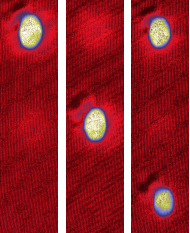
\includegraphics[scale=0.65]{Figures/TitlePicture.pdf} \\
\vspace{0.5em}
	
\includegraphics[width=0.5\textwidth]{Figures/Logo_Support.jpg}
\end{figure}

\vspace{-1em}

\begin{small}
\textbf{\textcolor{bellblue}{MACRO conference}}\\
\vspace{0em}
Newcastle, September 14th, 2016
\end{small}

\end{minipage}



\end{frame}

{
\usebackgroundtemplate{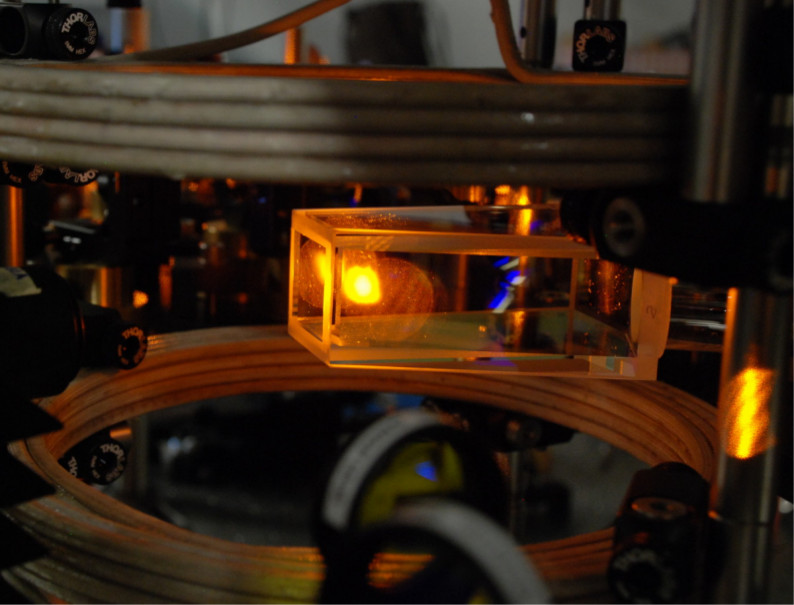
\includegraphics[width=\paperwidth]{Figures/MOT-picture.jpg}}
\begin{frame}[c,plain]

%\vspace{18em}
%
%\only<2>{
%\begin{flushright}
%\textcolor{white}{
%Easy to implement \& highly flexible\\
%\vspace{0.5em}
%Well defined interfaces, defects\\
%\vspace{0.5em}
%On-site properties control (resonance, loss) \\
%\vspace{0.5em}
%LDOS measurement \& direct imaging of the wavefunctions \\
%\vspace{0.5em}
%Transport measurement
%}
%\end{flushright}
%}

%\only<1->{
\btVFill{
\begin{flushright}
\textcolor{white}{\textbf{Our experimental setup to create \textcolor{bellblue}{sodium} BECs}}
\end{flushright}
}
%}

\end{frame}
}

\section{Introduction: Bose-Bose miscible mixture without buoyancy}
{
\usebackgroundtemplate{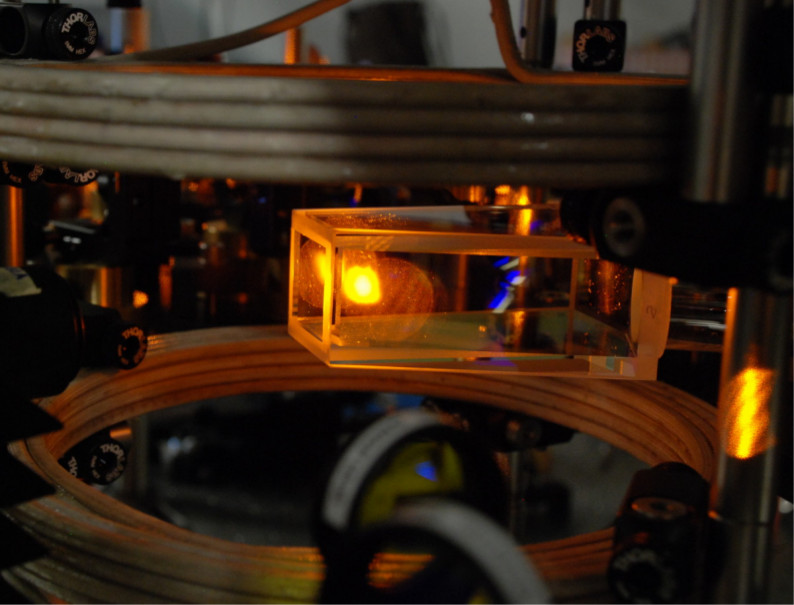
\includegraphics[width=\paperwidth]{Figures/MOT-picture.jpg}}
\begin{frame}<1-4>[t,plain,label=Outline]


\begin{minipage}[c][0.5\textheight][c]{\linewidth}
	\setbeamercolor{title}{fg=white,bg=bellblue}
	\only<1-3>{\pgfsetfillopacity{0.75}}
	\only<4->{\pgfsetfillopacity{0.35}}
	\hfill
	\begin{beamercolorbox}[wd=0.75\linewidth,center,colsep=0.5em,rounded=false]{title}
		\begin{center}
		\only<1-4>{\circled{white}{0.75}{1}\\}
		\only<5->{\circled{white}{0.35}{1}\\} 
		\vspace{1.5em}
		\textbf{Introduction} \\
		\vspace{1.5em}
		\end{center}
	\end{beamercolorbox}
	\hfill\hfill
\end{minipage}

\only<2->{
\begin{minipage}[c][0.5\textheight][c]{\linewidth}
	\setbeamercolor{title}{fg=white,bg=bellblue}
	\only<2,3>{\pgfsetfillopacity{0.75}}
	\only<5->{\pgfsetfillopacity{0.35}}
	\hfill
	\begin{beamercolorbox}[wd=0.75\linewidth,center,colsep=1em,rounded=false]{title}
		\begin{center}
		\only<2,3,5>{\circled{white}{0.75}{2}\\}
		\only<4,6->{\circled{white}{0.35}{2}\\}
		\vspace{1.5em}
		\textbf{Spin-Dipole polarizability} \\
		\vspace{1em}
		\end{center}
	\end{beamercolorbox}
	\hfill\hfill
\end{minipage}
}


\end{frame}
}
 %% OUTLINE 1/3
\begin{frame}
\frametitle{Introduction: Bose-Bose miscible mixture without buoyancy}
\setbeamercovered{invisible}


\begin{columns}[t]
\column{0.8\linewidth}
\begin{itemize}
\item 2-component BEC: 2 Zeeman levels $\ket{\uparrow}$, $\ket{\downarrow}$
\item Caracterized by scattering lengths:
	\begin{itemize}
		\item Intracomponent: $a_{\uparrow\uparrow}$, $a_{\downarrow\downarrow}$
		\item Intercomponent: $a_{\uparrow\downarrow}$
	\end{itemize}
\item Important property: miscibility if $a_{\uparrow\downarrow}<\sqrt{a_{\uparrow\uparrow}a_{\downarrow\downarrow}}$
\end{itemize}	
\column{0.2\linewidth}


\begin{figure}
\centering
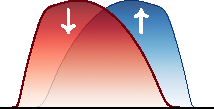
\includegraphics[scale=0.7]{Figures/Spinor_Illustration.pdf}
\end{figure}

\end{columns}

\begin{itemize}
\item Even when miscible: buoyancy problem in harmonic trap when $a_{\uparrow\uparrow} \neq a_{\downarrow\downarrow}$
\item It prevents the study of the static and dynamic response in harmonic trap
\end{itemize}
\begin{itemize}
\item Our system: $|3^2S_{1/2}, F=1, m_F=\pm1\rangle$ states of sodium 
\begin{figure}
\centering
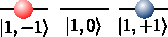
\includegraphics[scale=1.2]{Figures/Spinor_Scheme.pdf}
\end{figure}
\item Advantages
	\begin{itemize}
		\item Miscible
		\item Without buoyancy $a_{\uparrow\uparrow} = a_{\downarrow\downarrow} \equiv a$ 
		\item Close to the miscible/immiscible phase transition $(a-a_{\uparrow\downarrow})/a=0.07 \ll 1$
	\end{itemize}
\item Goals
\begin{itemize}
		\item Study the linear and dynamic response
		\item Observe that these properties are drastically modified close to the phase transition despite the weakly interacting nature of the gas
	\end{itemize}
\end{itemize}


\end{frame}

\begin{frame}
\frametitle{Spinor preparation}
\setbeamercovered{invisible}


\centering
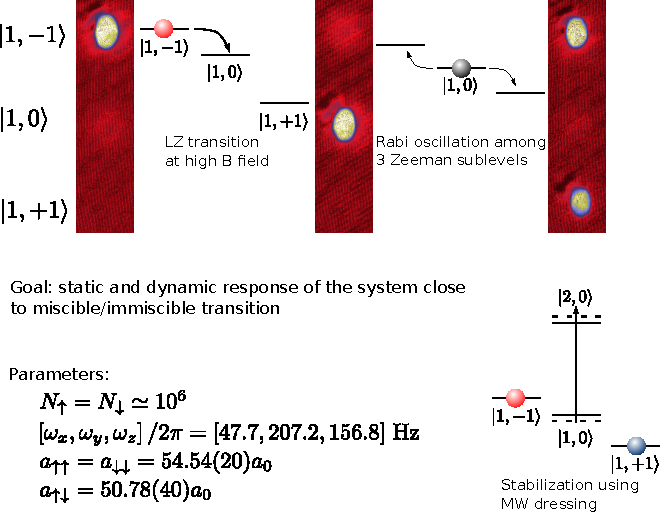
\includegraphics[width=0.9\linewidth]{Figures/Spinor_Preparation.pdf}


\end{frame}


	{%% OUTLINE 2/3
	\usebackgroundtemplate{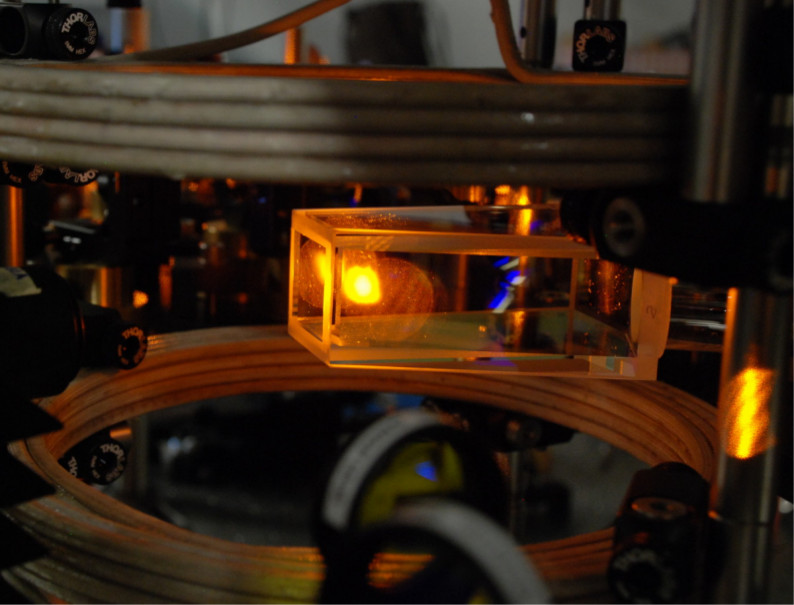
\includegraphics[width=\paperwidth]{Figures/MOT-picture.jpg}}
	\againframe<5>[t,plain]{Outline}
	}
\section{Spin-Dipole Polarizability}
\begin{frame}
\frametitle{Spin-Dipole Polarizability: static measurement}
\setbeamercovered{invisible}

\centering
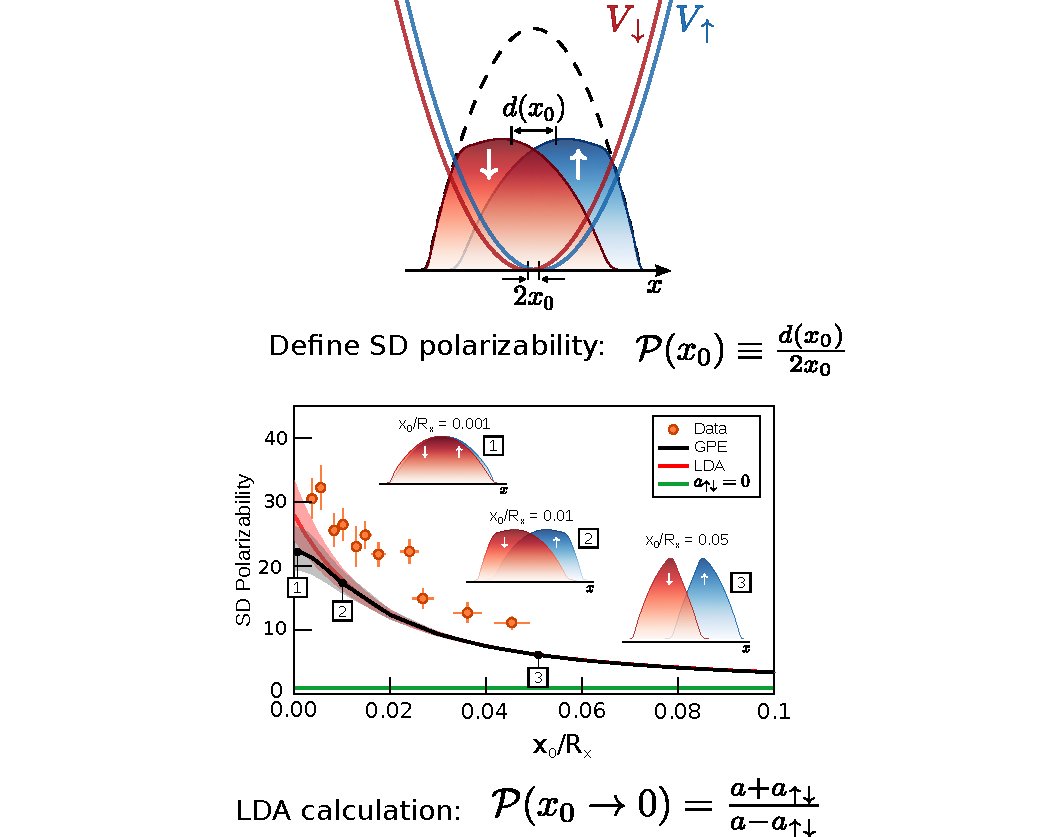
\includegraphics[width=0.9\linewidth]{Figures/SD_Polarizability2.pdf}

\end{frame}

	{%% OUTLINE 3/3
	\usebackgroundtemplate{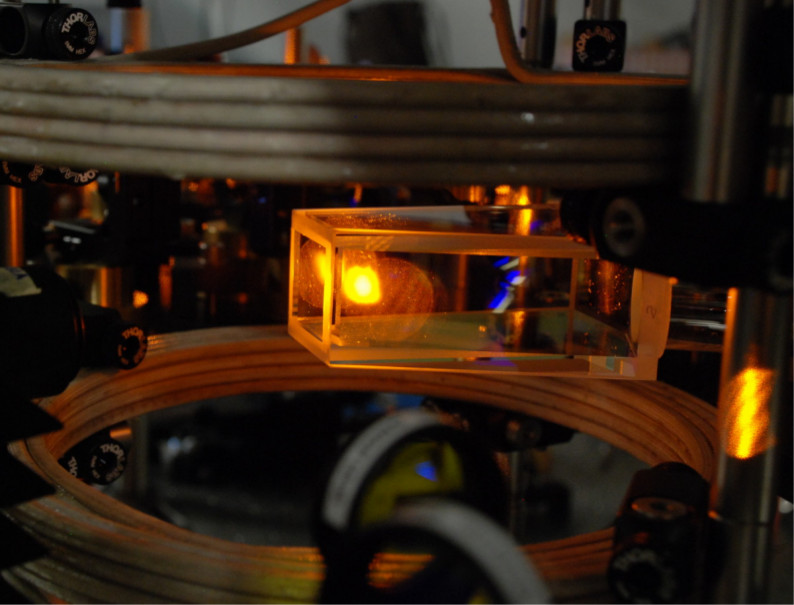
\includegraphics[width=\paperwidth]{Figures/MOT-picture.jpg}}
	\againframe<6>[t,plain]{Outline}
	}
\section{Spin-Dipole Oscillation}
\begin{frame}
\setbeamercovered{invisible}
\frametitle{Spin-Dipole Oscillation: dynamic measurement}

\centering
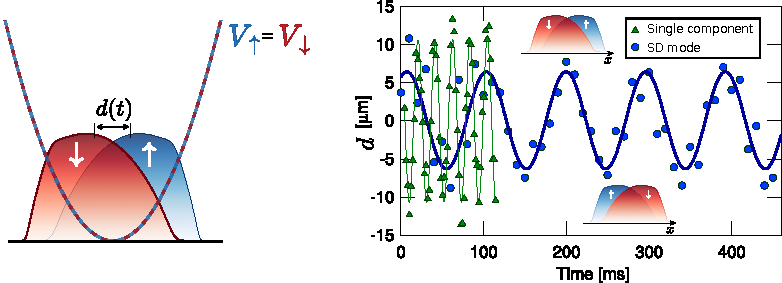
\includegraphics[width=0.95\linewidth]{Figures/SD_Oscillations2.pdf}

\begin{itemize}
\item We measure $\omega_{\text{SD}}/\omega_x = 0.218(2)$
	\begin{itemize}
	\item LDA $\omega_{\text{SD}} = 0.189(15) \omega_x$
	\item GPE $\omega_{\text{SD}} = 0.213(17) \omega_x$ 
	\end{itemize}
\item Sum rule approach links polarizability $\mathcal P$ and SD mode frequency $\omega_{\text{SD}}$: 
\begin{equation*}
\omega_{\text{SD}} = \frac{1}{\sqrt \mathcal P} \omega_x
\end{equation*}
%\item LDA prediction: 
%\begin{equation*}
%\omega_{\text{SD}} = \sqrt{\frac{a-a_{\uparrow\downarrow}}{a+a_{\uparrow\downarrow}}} \omega_x
%\end{equation*}
\end{itemize}

\end{frame}

\begin{frame}
\setbeamercovered{invisible}
\frametitle{Outlook}




\begin{columns}[t]
\column{0.5\linewidth}
\textcolor{bellblue}{Dynamical instability}
\begin{figure}
\centering
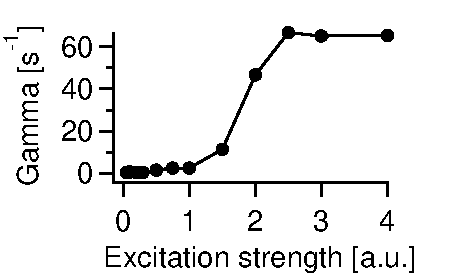
\includegraphics[width=0.6\linewidth]{Figures/Instability.pdf}
\end{figure}
\bellRef{M. Abad et al.}{EPJD}{2015}
\vspace{0.4cm}

\textcolor{bellblue}{Finite temperature (four fluid model)}
\begin{figure}
\centering
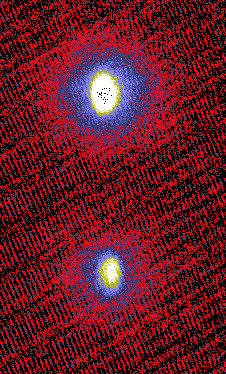
\includegraphics[width=0.3\linewidth]{Figures/Thermal_Spinor.jpg}
\end{figure}
\bellRef{J. Armqitis et al.}{PRA}{2015}\\
\bellRef{K. L. Lee et al.}{PRA}{2016}

	
\column{0.5\linewidth}
\textcolor{bellblue}{Magnetic soliton}
\begin{figure}
\centering
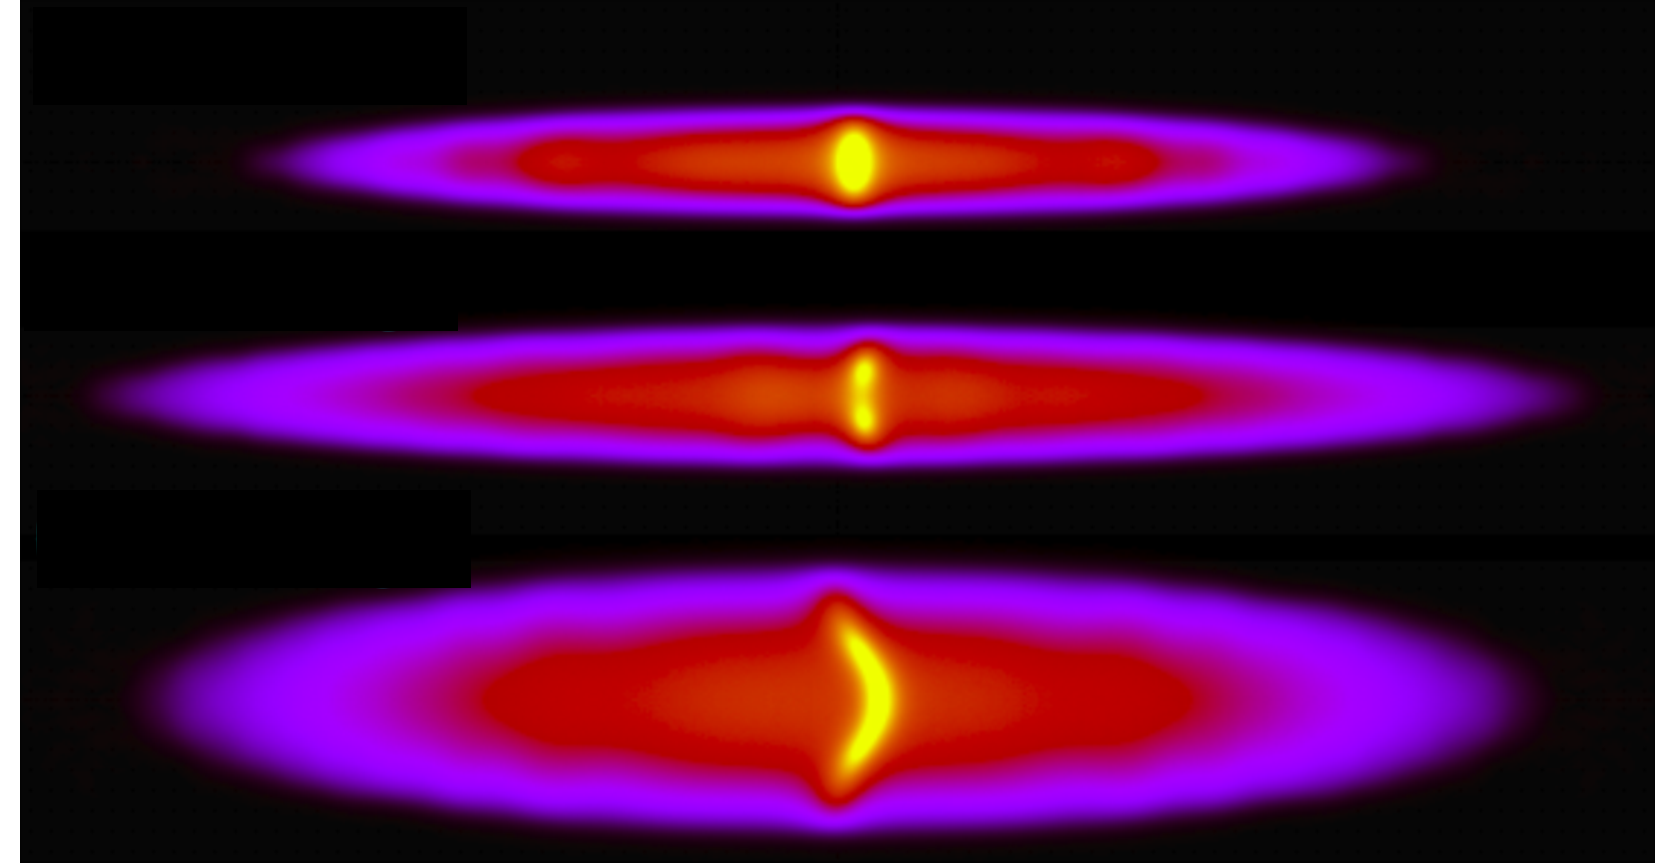
\includegraphics[width=0.67\linewidth]{Figures/magneticsoliton.pdf}
\end{figure}

\bellRef{C. Qu et al.}{PRL}{2016}



\vspace{0.4cm}


\textcolor{bellblue}{Coherent coupling between spin components}\\
Many references and ideas...
\begin{figure}
\centering
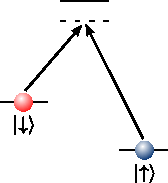
\includegraphics[width=0.4\linewidth]{Figures/Coherent_Coupling.pdf}
\end{figure}



\end{columns}


\end{frame}

\section{Conclusion}
{
\usebackgroundtemplate{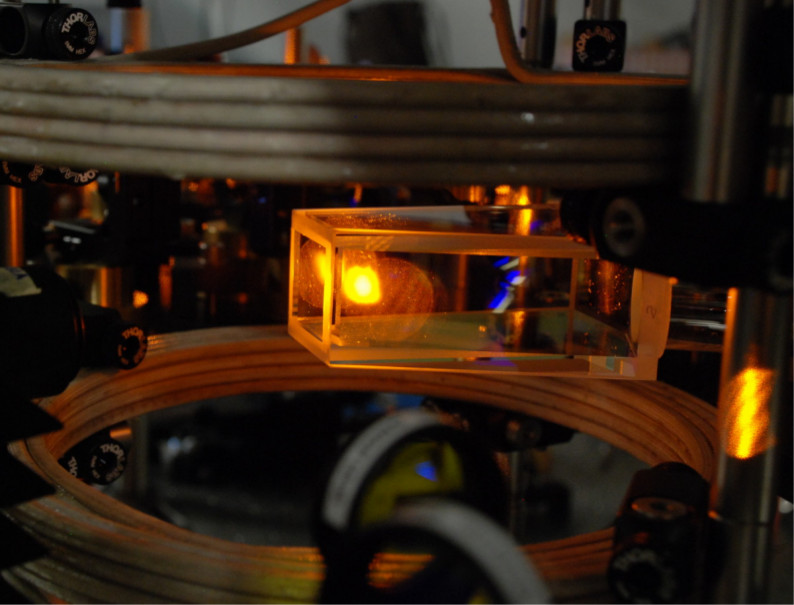
\includegraphics[width=\paperwidth]{Figures/MOT-picture.jpg}}
\begin{frame}<1-3>[t,plain]


\begin{minipage}[c][0.33\textheight][c]{\linewidth}
	\setbeamercolor{title}{fg=white,bg=bellblue}
	\only<1-4>{\pgfsetfillopacity{0.75}}
	\only<5->{\pgfsetfillopacity{0.35}}
	\hfill
	\begin{beamercolorbox}[wd=0.75\linewidth,center,colsep=0.5em,rounded=false]{title}
		\begin{center}
		\only<1-4>{\circled{white}{0.75}{1}\\}
		\only<5->{\circled{white}{0.35}{1}\\} 
		\vspace{1em}
		\textbf{New Bose-Bose mixture} \\
		\vspace{0.5em}
		{\small Miscible, without buoyancy, vicinity to the miscible/immiscible transition}
		\end{center}
	\end{beamercolorbox}
	\hfill\hfill
\end{minipage}

\only<2->{
\begin{minipage}[c][0.33\textheight][c]{\linewidth}
	\setbeamercolor{title}{fg=white,bg=bellblue}
	\only<2,3,5>{\pgfsetfillopacity{0.75}}
	\only<4,6->{\pgfsetfillopacity{0.35}}
	\hfill
	\begin{beamercolorbox}[wd=0.75\linewidth,center,colsep=1em,rounded=false]{title}
		\begin{center}
		\only<2,3,5>{\circled{white}{0.75}{2}\\}
		\only<4,6->{\circled{white}{0.35}{2}\\}
		\vspace{1em}
		\textbf{SD polarizability and oscillation} \\
		\vspace{0.5em}
		{\small Close to the transition: large polarizability, softening of the SD mode.}
		\end{center}
	\end{beamercolorbox}
	\hfill\hfill
\end{minipage}
}

\only<3>{
\begin{minipage}[c][0.33\textheight][c]{\linewidth}
\centering
\textcolor{white}{
\textbf{More info}: 
Arxiv:1607.04574 (2016) \\
\vspace{1em}
\textbf{mail}: tom.bienaime@unitn.it -- \textbf{web}: http://bec.science.unitn.it/
}
\end{minipage}
}
\end{frame}
}

\begin{frame}
\frametitle{Acknowledgments}

\begin{columns}[b]


\column[b]{0.5\linewidth}

\begin{itemize}
\item BEC \textcolor{bellblue}{experiment} $@$ Trento\\
\vspace{0.5em}
T. Bienaimé\\
E. Fava\\
G. Colzi\\
C. Mordini\\
S. Serafini\\
G. Lamporesi\\
G. Ferrari\\

\item \textcolor{bellblue}{Theoretical} study $@$ Trento\\
\vspace{0.5em}
C. Qu \\
S. Stringari

\vspace{1em}

\end{itemize}

\column[b]{0.5\linewidth}

\begin{figure}
\centering
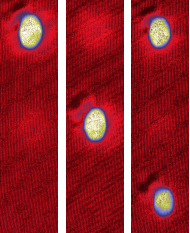
\includegraphics[width=0.55\textwidth]{Figures/TitlePicture.pdf}
\end{figure}

\end{columns}

\begin{itemize}
\item \textcolor{bellblue}{Funding} $\&$ \textcolor{bellblue}{Support}\\
\end{itemize}
\begin{figure}
\centering

\includegraphics[width=0.65\textwidth]{Figures/Logo_Support.jpg}
\end{figure}

\vspace{0em}
\begin{center}
{\Large \textcolor{bellblue}{\textbf{Thank you for your attention !}}}	 
\end{center}

\end{frame}







\end{document}


